\section{Problems}

\subsection{[Basic Statistics]}

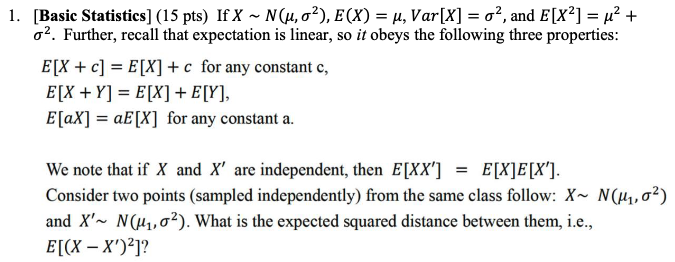
\includegraphics[width=1\textwidth]{media/hw2_q1.png}

We are given $E[(X-X')^2]$. Let's expand this.
\begin{align}
    E[(X-X')^2] &= E[(X-X')(X-X')] \nonumber \\
    &= E[X^2 - 2XX' + X'^2] \nonumber \\
    &= E[X^2] - E[2XX'] + E[X'^2 ] && \text{using linearity property} \label{q1_1}
\end{align}

We are given $E[XX']=E[X]E[X']$, given $X$ and $X'$ are independent. Using this, and the second expectation property, we substitute back into Eq. \ref{q1_1}:
\begin{align}
    E[(X-X')^2] &= E[X^2] - 2 E[XX'] + E[X'^2 ] \nonumber \\
    &= E[X^2] - 2 E[X]E[X'] + E[X'^2 ] \label{q1_2}
\end{align}

We are also given $E[X^2]=\mu^2 + \sigma^2$, and $E[X]=\mu$. Substituting these back into Eq. \ref{q1_2}, we have:
\begin{align}
    E[(X-X')^2] &= (\mu_X^2 + \sigma_X^2) - 2\mu_X \mu_{X'} + (\mu_{X'}^2 + \sigma_{X'}^2) \label{q1_3}
\end{align}

Remember that both $X$ and $X'$ are independently sampled from the same class: $X, X' \sim N(\mu, \sigma^2)$. Therefore we let $\mu_X = \mu_{X'}$, and $\sigma_X = \sigma_{X'}$. Then Eq. \ref{q1_3} becomes:
\begin{align}
    E[(X-X')^2] &= \mu^2 + \sigma^2 - 2\mu^2 + \mu^2 + \sigma^2 \nonumber \\
    &= 2\mu^2 - 2\mu^2 + 2\sigma^2 \nonumber \\
    &= 2\sigma^2 \label{q1_4}
\end{align}

$\therefore$ The expected squared distance between $E[(X-X')^2]$ is $2\sigma^2$ (which also makes intuitive sense).

\subsection{[Basic Linear Algebra] (15 pts) We are given a vector $x = [0, 0.2, 1.0, 2.2]$. Which of the following vector is closest to $x$ and what is the distance from the closest point to $x$ under each of the following vector norms?}

$$x_1 = [0.7, 0.2, 0.5, 2.0]$$
$$x_2 = [0, 1.0, 1.5, 2.2]$$
$$x_3 = [0.8, 0.1, 1.2, 2.0]$$

a) 0-norm =
b) 1-norm =
c) 2-norm =
d) $\infty$-norm =

\subsubsection{For $\mathbf{x_1}$:}
\begin{align}
    ||\mathbf{x} - \mathbf{x_1}|| &= 
    \begin{bmatrix}
        |0 - 0.7| & |0.2 - 0.2| & |1 - 0.5| & |2.2 - 2|
    \end{bmatrix} \nonumber \\
    &= 
    \begin{bmatrix}
        0.7 & 0 & 0.5 & 0.2
    \end{bmatrix} 
\end{align}
\begin{align}
    \Rightarrow ||\mathbf{x_1}||_0 &= 3
\end{align}
\begin{align}
    \Rightarrow  ||\mathbf{x_1}||_1 &= \sum ||\mathbf{x} - \mathbf{x_1}|| = 0.7 + 0 + 0.5 + 0.2 = 1.4
\end{align}
\begin{align}
    \Rightarrow ||\mathbf{x_1}||_2 &= \sqrt{|0 - 0.7|^2 + |0.2 - 0.2|^2 + |1 - 0.5|^2 + |2.2 - 2|^2} \nonumber \\
    &= \sqrt{0.7^2 + 0^2 + 0.5^2 + 0.2^2} = \sqrt{0.78} = 0.8832
\end{align}
\begin{align}
    \Rightarrow ||\mathbf{x_1}||_{\infty} &= max ||\mathbf{x} - \mathbf{x_1}|| = 0.7
\end{align}

\subsubsection{For $\mathbf{x_2}$:}
\begin{align}
    ||\mathbf{x} - \mathbf{x_2}|| &= 
    \begin{bmatrix}
        |0 - 0| & |0.2 - 1| & |1 - 1.5| & |2.2 - 2.2|
    \end{bmatrix} \nonumber \\
    &= 
    \begin{bmatrix}
        0 & 0.8 & 0.5 & 0
    \end{bmatrix} 
\end{align}
\begin{align}
    \Rightarrow ||\mathbf{x_2}||_0 &= 2
\end{align}
\begin{align}
    \Rightarrow  ||\mathbf{x_2}||_1 &= \sum ||\mathbf{x} - \mathbf{x_2}|| = 0 + 0.8 + 0.5 + 0 = 1.3
\end{align}
\begin{align}
    \Rightarrow ||\mathbf{x_2}||_2 &= \sqrt{|0 - 0|^2 + |0.2 - 1|^2 + |1 - 1.5|^2 + |2.2 - 2.2|^2} \nonumber \\
    &= \sqrt{0^2 + 0.8^2 + 0.5^2 + 0^2} = \sqrt{0.89} = 0.9434
\end{align}
\begin{align}
    \Rightarrow ||\mathbf{x_2}||_{\infty} &= max ||\mathbf{x} - \mathbf{x_2}|| = 0.8
\end{align}

\subsubsection{For $\mathbf{x_3}$:}
\begin{align}
    ||\mathbf{x} - \mathbf{x_3}|| &= 
    \begin{bmatrix}
        |0 - 0.8| & |0.2 - 0.1| & |1 - 1.2| & |2.2 - 2|
    \end{bmatrix} \nonumber \\
    &= 
    \begin{bmatrix}
        0.8 & 0.1 & 0.2 & 0.2
    \end{bmatrix} 
\end{align}
\begin{align}
    \Rightarrow ||\mathbf{x_3}||_0 &= 4
\end{align}
\begin{align}
    \Rightarrow  ||\mathbf{x_3}||_1 &= \sum ||\mathbf{x} - \mathbf{x_2}|| = 0.8 + 0.1 + 0.2 + 0.2 = 1.3
\end{align}
\begin{align}
    \Rightarrow ||\mathbf{x_3}||_2 &= \sqrt{|0 - 0.8|^2 + |0.2 - 0.1|^2 + |1 - 1.2|^2 + |2.2 - 2|^2} \nonumber \\
    &= \sqrt{0.8^2 + 0.1^2 + 0.2^2 + 0.2^2} = \sqrt{0.73} = 0.8544
\end{align}
\begin{align}
    \Rightarrow ||\mathbf{x_3}||_{\infty} &= max ||\mathbf{x} - \mathbf{x_3}|| = 0.8
\end{align}

Based on the above norm calculations, we have the following results:
\begin{enumerate}
    \item by the 0-norm, $\mathbf{x_2}$ is the closest to $\mathbf{x}$.
    \item by the 1-norm, both $\mathbf{x_2}$ and $\mathbf{x_3}$ are the closest to $\mathbf{x}$.
    \item by the 2-norm, $\mathbf{x_3}$ is the closest to $\mathbf{x}$.
    \item by the $\infty$-norm, $\mathbf{x_1}$ is the closest to $\mathbf{x}$.
\end{enumerate}

\subsection{[Convexity] (1)}

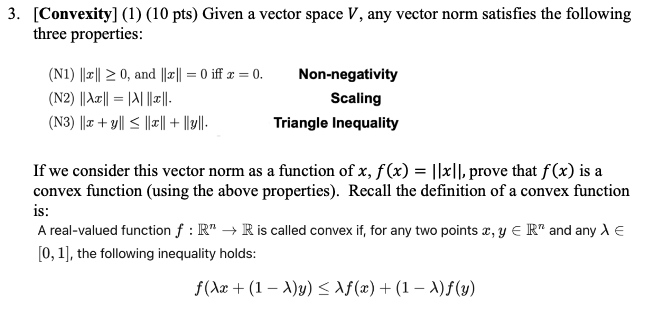
\includegraphics[width=1\textwidth]{media/hw2_q3.png}

We are given the definition of a convex function:
\begin{align}
    f(\lambda x + (1-\lambda)y) \leq \lambda f(x) + (1-\lambda) f(y) \label{convexity}
\end{align}

We start with $f(x) = ||x||$:
\begin{align}
    f(x) &= ||x|| \nonumber \\
    &= f(\lambda x + (1-\lambda)y) \nonumber \\
    &= ||\lambda x + (1-\lambda)y|| && \text{using Eq. \ref{convexity}} \nonumber \\
    &\leq ||\lambda x || + ||(1-\lambda) y|| && \text{using triangle inequality} \nonumber \\
    &= |\lambda | ||x|| + |(1-\lambda)| ||y|| && \text{using scaling} \label{q3_2}
\end{align}

Then using Eq. \ref{q3_2}, and substituting back into the convex function (Eq. \ref{convexity}), we have:
\begin{align}
    f(\lambda x + (1-\lambda)y) &= ||\lambda x || + ||(1-\lambda) y|| \leq |\lambda | ||x|| + |(1-\lambda)| ||y|| \label{q3_3}
\end{align}

$\therefore$ We have shown that the vector norm as a function, $f(x) = ||x||$, is indeed convex, as it satisfies the inequality of the convex function (Eq. \ref{convexity}).

\subsection{[Convexity] (2) (10 pts). Prove that the convexity is preserved under a linear transformation. Supposed $f(w)$ is convex in terms of $w$. Prove that $g(w)=f(X w + b)$ is also convex in terms of $w$ where $X$ is a fixed matrix of appropriate size, and $b$ is a fixed vector of appropriate size. (So $X$ and $b$ are not variables in $g$). (Hint: you can simply use the definition of convex function)}

Once again, we will use the convex function definition, Eq. \ref{convexity} from the previous question. We will re-write Eq. \ref{convexity} in terms of $g(w)$:

\begin{align}
    g(\lambda x + (1-\lambda)y) \leq \lambda g(x) + (1-\lambda) g(y) \label{q4_1}
\end{align}

Let's examine the RHS of Eq. \ref{q4_1}, and substitute $g(w) = f(Xw+b)$:
\begin{align}
    \lambda g(x) + (1-\lambda) g(y) &= \lambda f(Xw_1+b) + (1-\lambda) f(Xw_2+b) \label{q4_2} \nonumber \\
    &= f(\lambda X w_1 + (1-\lambda) X w_2 + b)
\end{align}

Let's check the convexity of Eq. \ref{q4_2}:
\begin{align}
    f(\lambda X w_1 + (1-\lambda) X w_2 + b) &\leq \lambda f(X w_1 +b) + (1-\lambda) f(X w_2 + b) \label{q4_3} \nonumber \\
    &= \lambda g(x) + (1-\lambda) g(y)
\end{align}

Finally we substitute Eq. \ref{q4_3} into Eq. \ref{q4_2}:
\begin{align}
    g(\lambda x + (1-\lambda)y) &\leq \lambda g(x) + (1-\lambda) g(y) \label{q4_4}
\end{align}

$\therefore$ Convexity is preserved under the linear transformation $g(w)=f(X w + b)$.

\subsection{[Convexity] (3) (10 pts). From (1) and (2), prove the “loss” function $||y-Xw||_2$ is convex in terms of $w$ where $X_{n \times d}$ is a data matrix containing $n$ examples and each example has $d$ features, and $y$ is a column vector of length $d$. This dataset has been observed and thus fixed, and $w$ is the only variable in the norm.}

Let's represent the loss function by a vector $\mathbf{a}$, where $\mathbf{a} = y - Xw$. Then we have:
\begin{align}
    f(x) &= \mathbf{a} \nonumber \\
    &= y-Xw
\end{align}

The norm of this vector $\mathbf{a}$ satisfies the vector norm properties, and is given by:
\begin{align}
    ||\mathbf{a}|| &= || y-Xw || \nonumber \\
    \Rightarrow ||\mathbf{a}||_2 &= \sqrt{\sum_{i=1}^n \mathbf{a}_i^2}
\end{align}

As shown in Eq. \ref{q3_3} in Question 2.3, the vector norm $||\mathbf{a}||$ is indeed convex. \\

Similarly, let $g(w)=f(y-Xw)$. As shown in Eq. \ref{q4_4}, this linear transformation is also convex. \\

Therefore we have shown that a function in the form of a linear norm ($||y-Xw||_2$) is convex.
